\documentclass[a4paper, 11pt]{article}
\title{Jerry Trader Documentation}
\author{JerryHong}
\date{March 2026}
\date{Started December 2025 \\ Last updated: \today}

\usepackage{fontspec}
\usepackage{xeCJK} % for support Chinese.
% Set a CJK monospaced font if available (silences xeCJK unknown-tt warning).
\setCJKmainfont{Microsoft YaHei}
\setCJKmonofont{Microsoft YaHei}
\usepackage{xcolor}
\usepackage{graphicx}
\usepackage{tabularx}
\usepackage{ragged2e}
\usepackage{array}
\usepackage{seqsplit}
\usepackage{fvextra}
\usepackage{enumitem}
\newcolumntype{Y}{>{\RaggedRight\arraybackslash}X}
% (removed global \texttt redefinition - use \seqsplit manually where needed)

\begin{document}
\maketitle

\pagebreak

\tableofcontents

\pagebreak

\section{Introduction}

\paragraph{Summary}
Jerry Trader is a quant trading platform mainly focus on real-time US pre-market penny stock break out momentum trading strategy,
written multi-language (Python + Rust + React).
This documentation provides an overview of the app's features, architecture, and usage instructions \begin{em}based on my trading strategies\end{em}.

The project follows a monorepo layout:

\begin{itemize}
\item \texttt{python} --- Python backend (orchestration, I/O, backend services)
\item \texttt{rust} --- Rust computation core (compiled via maturin/PyO3 as \texttt{\seqsplit{jerry\_trader.\_rust}})
\item \texttt{frontend} --- React + TypeScript frontend (Vite)
\end{itemize}

\paragraph{Strategy}
Here is a summary of my strategy based on emperical trading experience, and the modules are designed to better validate, automate this strategy:

\begin{itemize}

\item Entry Attention Condition:\\
when tickers are getting active, it has a amount of gains suddenly, we do the momentum trading.
for my current project, I use Top20 Entry as a detector.

\item It's Better If:
\begin{itemize}
    \item it has recent hot news with it.
    \item the float shares are relatively low, below 20M is preferred.
    \item the country location is better not foreign-registered, etc.
    \item price is preferred \$1--\$20
    \item the market has all the attention on this one.
    \item Order Book liquidity good(intense trade rates with good up-rising momentum)
\end{itemize}

\item It's Better NOT If:
\begin{itemize}
    \item Order Book liquidity good but with multiple key-level rejections.
    \item price under 0.5
    \item big cap companies earnings beat.
\end{itemize}

\end{itemize}

It's not saying that if all the conditions fit it will definitly be a good trade.
the conditions will be better if all fit, but sometimes there are unknown black swarn ones, so
the key metrics will still be price-volume action and orderbook analysis etc.and besides of that,
for a long-term profitable trading strategy, also it depends your trading execution and risk management like:

\begin{itemize}
    \item entry timing and price.
    \item risk management(marginal account risk etc).
    \item \ldots
\end{itemize}

\paragraph{Feature}
for current version, here are some features that done:
\begin{itemize}
    \item modules decoupled, driven by redis stream msg.
    \item rank list column and overview chart for top20 tickers visualization.
    \item instant news data fetch, process, LLM system prompt sentiment process, persistence.
    \item stock info data like: float data, basic information fetch, process, persistence.
    \item ibkr order execution,management,persistence to PostgreSQL.
    \item real-time bar build and persistence optimized using clickhouse\&rust.
    \item live mode and replay mode support.
    \item rust based global clock for time accuracy.
\end{itemize}

\pagebreak

\section{Frontend Modules}
\subsection{frontend overview}

\begin{figure}[!ht]
\centering
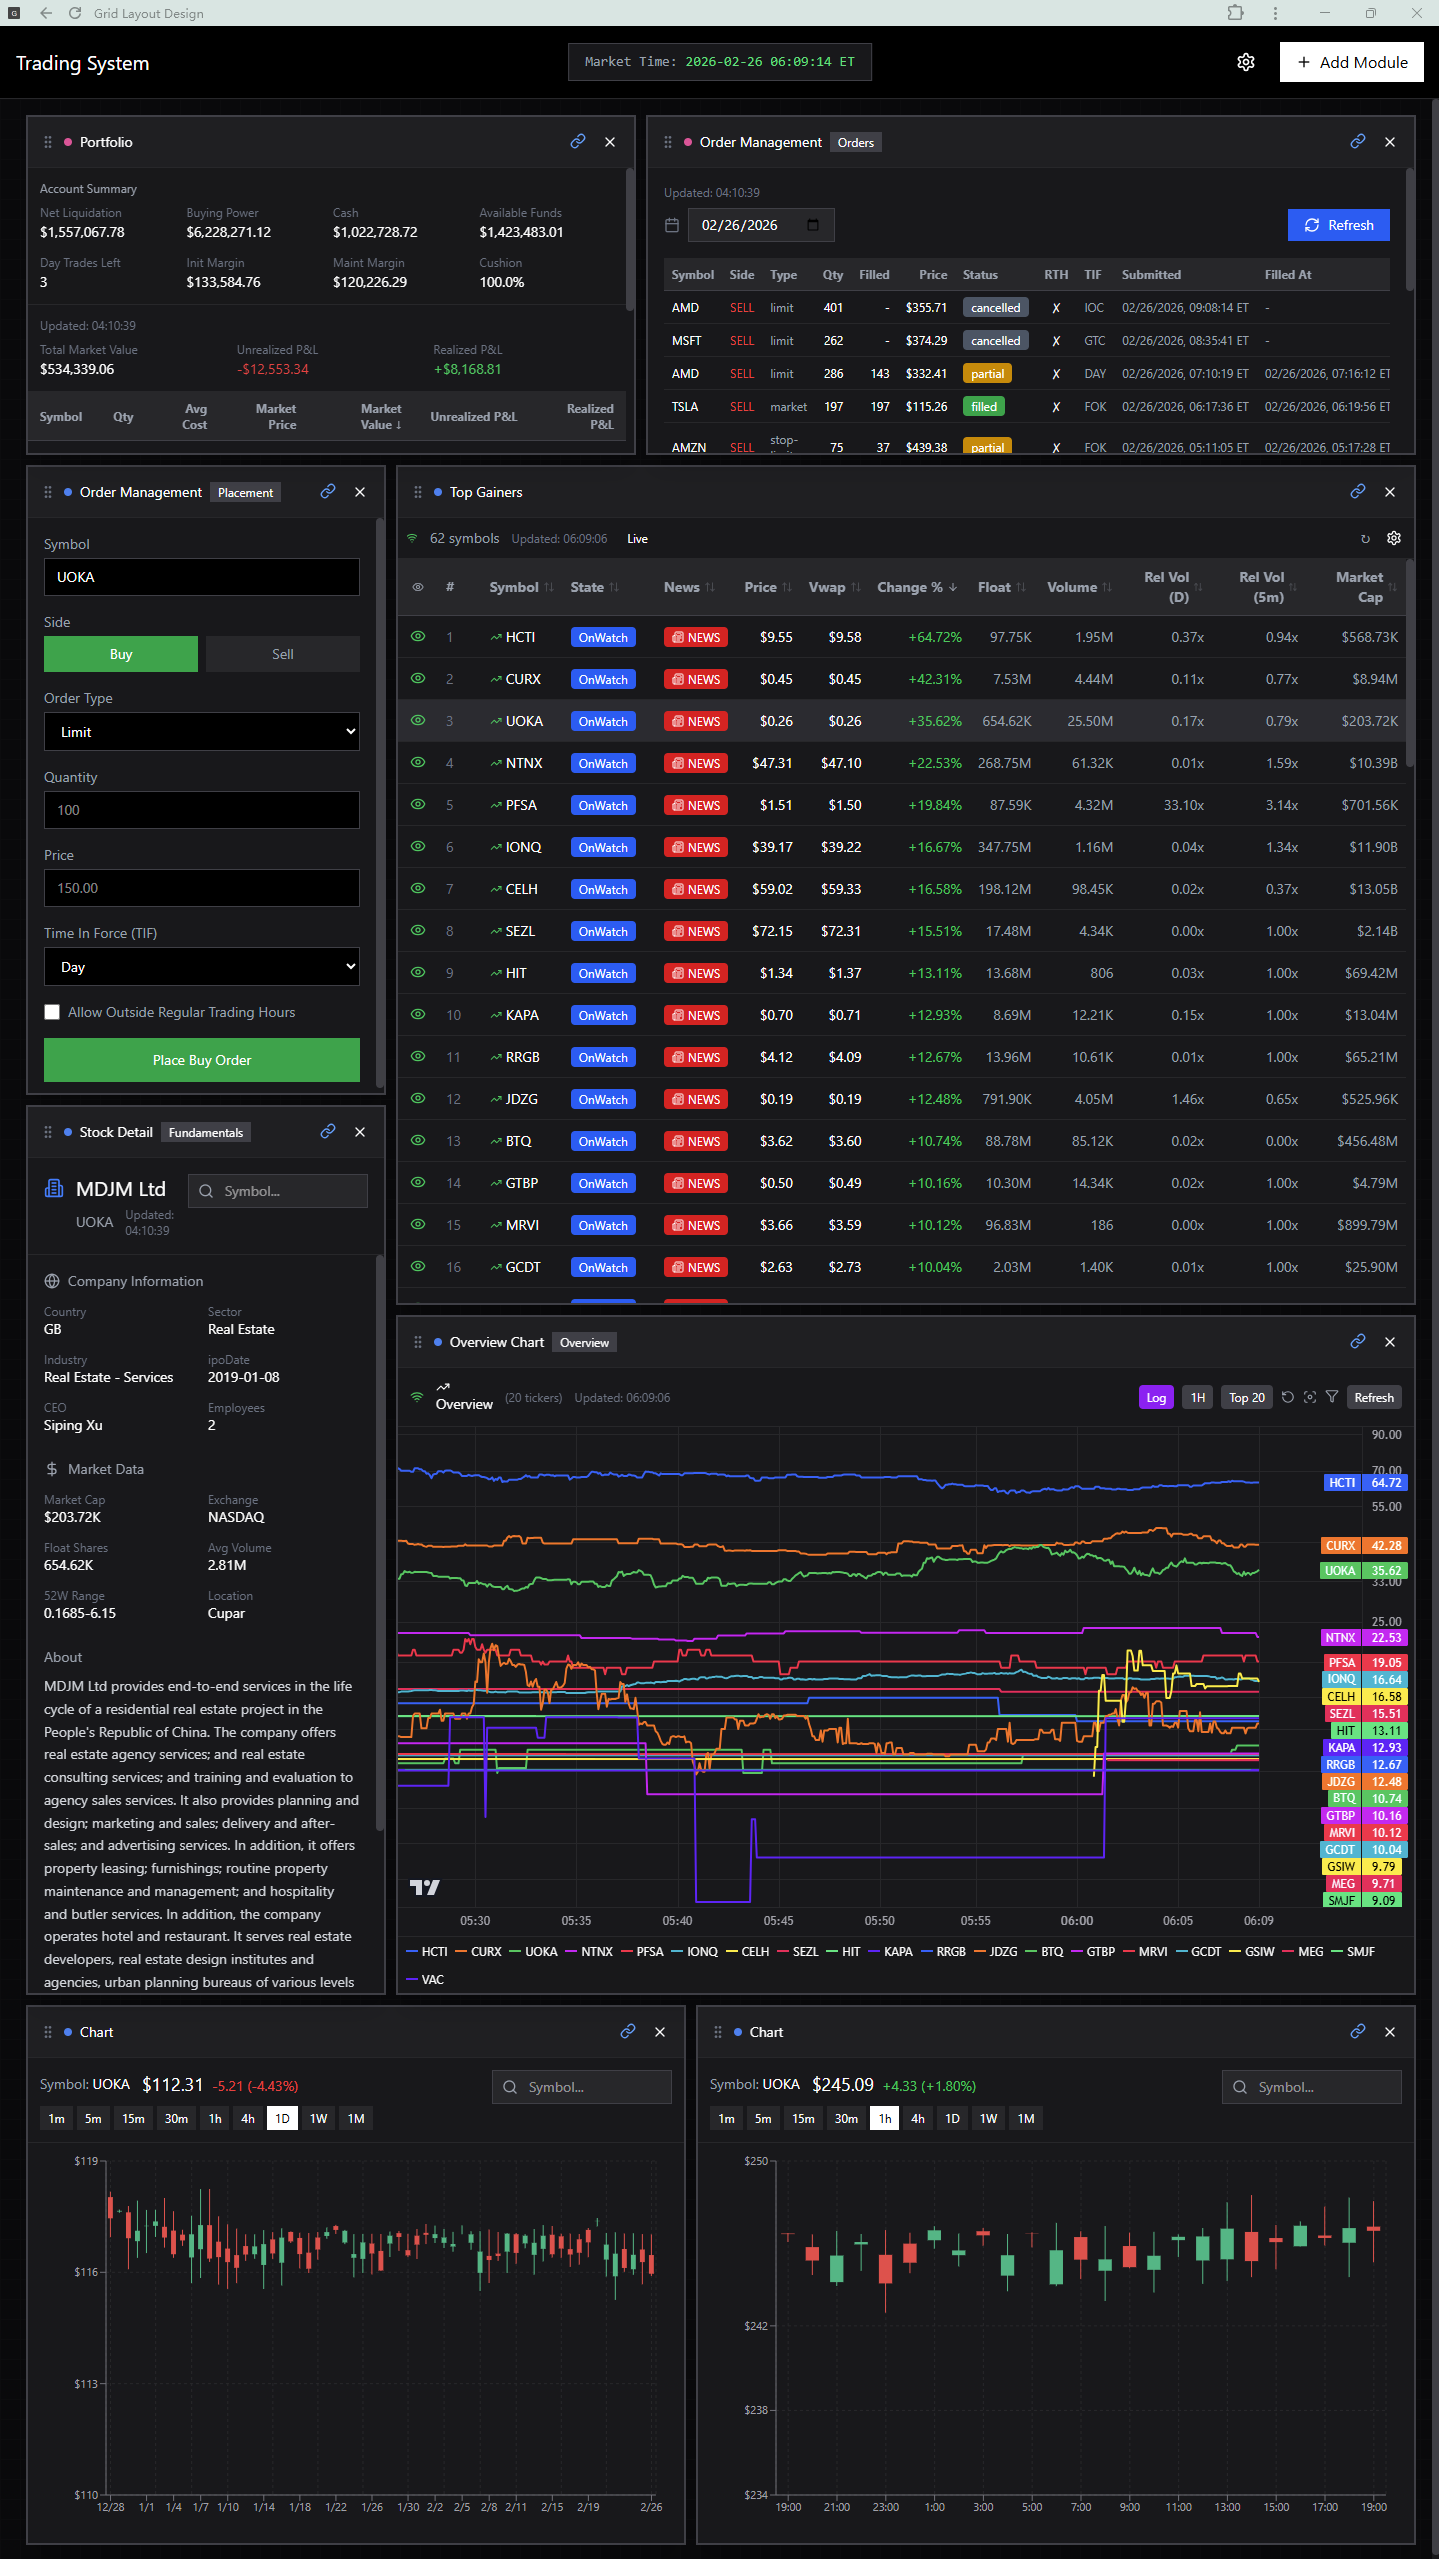
\includegraphics[width=0.8\textwidth]{../assets/JerryTrader.png}
\caption{Jerry Trader Application Interface}
\label{fig:jerrytrader}
\end{figure}

\paragraph{Platform Overview}
So, as you can see above, this is my current version of frontend web app interface.
but you might wonder, as a rigorous quant trading platform, why would I develop a trading platform that UI is designed for human-centered trade execution?\\
well, first, I just love trade, my goal is to be profitable quant trader, not researcher due to my lack of rigourous knowlegde of mathematics.
second, this project is planned for long-term architecture, I don't have the experience and ability
to develop a end-to-end tickdata to machine-decision execution quant platform. the graduate approach is the only choice.

\subsection{modules breakdown}

\begin{table}[!htbp]
\centering
\footnotesize
\renewcommand{\arraystretch}{1.05}
    \begin{tabularx}{\textwidth}{|>{\RaggedRight\arraybackslash}p{2.5cm}|>{\RaggedRight\arraybackslash}p{2.5cm}|Y|Y|}
\hline
\textbf{Module Type} & \textbf{Sub-View Name} & \textbf{Description} & \textbf{Backend} \\
\hline
rank-list &  & rank list with key metrics & \seqsplit{core.snapshot, static-data-worker, news-worker, core.signals} \\
\hline
stock-detail & fundamentals & stock basic info & \seqsplit{staticdata-worker} \\
\hline
stock-detail & news &  & \seqsplit{news-worker} \\
\hline
overview-chart & overview &  & \seqsplit{overviewchart-management} \\
\hline
overview-chart & focus & focus on one tiker with state segmentation & \seqsplit{overviewchart-management} \\
\hline
chart &  &  & \seqsplit{chart-data-service} \\
\hline
portfolio &  & portfolio and positions & OrderManagement \\
\hline
order-management & placement &  & OrderManagement \\
\hline
order-management & orders &  & OrderManagement \\
\hline
\end{tabularx}
\caption{Module descriptions and their corresponding backends.}
\label{tab:module_descriptions}
\end{table}

In the next Chapter, I will break down the details of each module in the above table, which will include:
\begin{itemize}
    \item data preparation
    \item data process
    \item orchestration
    \item module design
\end{itemize}

\pagebreak

\section{Backend Architecture}

\emph{not start to rewind yet. below is just lagacy llm-generated notes\&summary}

\subsection{Package Layout}
The Python backend is organized into the following top-level packages:

\subsection{Computation Core (\texttt{core/})}
The \texttt{core/} package is the \textbf{Rust migration boundary}. Each subpackage follows a compute/orchestration split:

\begin{itemize}
    \item \texttt{compute.py} --- Pure functions \& stateful trackers (\textbf{Rust migration target}). These have planned counterparts in \texttt{rust/src/}.
    \item \texttt{processor.py} / \texttt{engine.py} --- I/O orchestration (Redis, InfluxDB, threads). Stays in Python.
\end{itemize}

The \texttt{\_bridge.py} module provides a try/except dispatch:
\begin{Verbatim}[breaklines=true]
try:
    from jerry_trader._rust import VolumeTracker, compute_ranks
except ImportError:
    from jerry_trader.core.snapshot.compute import VolumeTracker, compute_ranks
\end{Verbatim}

\noindent This allows incremental migration --- Rust implementation when compiled, Python fallback otherwise.

\subsection{Services}

{\small\RaggedRight
\begin{itemize}[leftmargin=*,labelsep=6pt]
    \item \textbf{BackendForFrontend (BFF)} \\
    FastAPI + WebSocket server running on the main machine. Collects and pre-processes (\texttt{\seqsplit{core.snapshot}}); receives and emits rank data and overview-chart data to the frontend.

    \item \textbf{core.snapshot (SnapshotProcessor)} \\
    Receives raw market snapshots from Redis stream, computes ranks and derived metrics (via Rust when available), manages the top-movers subscription set, writes to output Redis stream and InfluxDB.

    \item \textbf{core.factors (FactorManager)} \\
    {\scriptsize\RaggedRight Real-time factor engine. Ingests tick-level trade data.
    Computes trade rate. Computes acceleration. Produces rolling z-scores.
    Outputs to InfluxDB. Uses Redis (HSET) for metadata. Includes historical bootstrap via Polygon API.\par}\justifying

    \item \textbf{core.signals (StateEngine)} \\
    Polls factor HSETs and fires state transition events (QUIET $\to$ ACTIVE, ACTIVE $\to$ QUIET) based on z-score thresholds.

    \item \textbf{core.news (NewsProcessor)} \\
    LLM-based news classification. Determines if news articles are positive catalysts using DeepSeek API.

    \item \textbf{OrderManagement} \\
    Order management system based on Interactive Brokers API. Handles order placement, status callbacks, portfolio and position tracking. Backed by PostgreSQL via SQLAlchemy + Alembic.

    \item \textbf{DataSupply} \\
    External data sources:
    \begin{itemize}
        \item \texttt{snapshotDataSupply} --- market snapshot collection \& replay
        \item \texttt{tickDataSupply} --- real-time tick data (Polygon.io, ThetaData, local Rust replay)
        \item \texttt{staticdataSupply} --- fundamentals, borrow fee, news fetch
        \item \texttt{bootstrapdataSupply} --- historical data loaders
    \end{itemize}

    \item \textbf{DataManager} \\
    Data-serving workers that bridge DataSupply to the BFF:
    \begin{itemize}
        \item \texttt{\seqsplit{static\_data\_worker}} --- fetches fundamentals for subscribed tickers
        \item \texttt{\seqsplit{news\_worker}} --- fetches and caches news
        \item \texttt{\seqsplit{tickdata\_server}} --- serves tick data to frontend and factor engine
        \item \texttt{\seqsplit{chart\_data\_service}} --- historical bar data for TradingView chart
    \end{itemize}

    \item \textbf{utils} \\
    Cross-cutting utilities: config, logger, Redis key naming, session management, path resolution.
\end{itemize}
\par}

\pagebreak

\subsection{Rust Migration Roadmap}
\label{sec:rust-roadmap}
The migration from Python \texttt{compute.py} modules to Rust follows a three-step progression, ordered from simplest to most complex:

\begin{enumerate}
    \item \textbf{Step 1: Pure math functions} (\texttt{core/factors/compute.py}) \\
    \texttt{z\_score} and \texttt{price\_accel} --- stateless, no external dependencies.
    This step establishes the full end-to-end workflow: write Rust in \texttt{\seqsplit{lib.rs}},
    run \texttt{maturin develop}, \texttt{\seqsplit{\_bridge.py}} auto-switches,
    existing tests validate correctness, \texttt{RUST\_FACTORS} flips to \texttt{True}.

    \item \textbf{Step 2: Stateful tracker} (\texttt{core/snapshot/compute.py}) \\
    \texttt{VolumeTracker} as a \texttt{\#[pyclass]} with methods ---
    learn stateful Rust objects exposed to Python via PyO3.

    \item \textbf{Step 3: DataFrame operations} (\texttt{core/snapshot/compute.py}) \\
    \texttt{\seqsplit{compute\_ranks}}, \texttt{\seqsplit{compute\_derived\_metrics}}, \texttt{\seqsplit{compute\_weighted\_mid\_price}}
    --- Polars DataFrame in/out, requires the \texttt{pyo3-polars} crate. Most complex.
\end{enumerate}

\noindent\textbf{Note:} \texttt{core/signals/} (StateEngine) is excluded from the Rust migration roadmap.
The signal/state detection logic depends on strategy rules that are not fully decided yet;
it will remain Python-only for the foreseeable future.

\noindent\textbf{Status:} Step~1 completed. \texttt{z\_score} achieved 3.6--10.7$\times$ speedup,
\texttt{price\_accel} achieved 8.9--12.1$\times$ speedup over Python.
Steps~2--3 are deferred in favour of the Bars Builder pipeline below.

\pagebreak

\subsection{Stage 2.5 --- Bars Builder Pipeline}
\label{sec:bars-builder}

The Chart module requires a reliable server-side bar-building pipeline.
The v1.0 architecture (frontend fetches historical bars from Polygon API, real-time
last-bar-only update from raw trade ticks in \texttt{chartDataStore.ts}) suffered from:
\begin{itemize}[nosep]
    \item Bar consistency issues across timeframes
    \item Duplicated aggregation logic (frontend \emph{and} factor engine)
    \item No single source of truth for completed bars
    \item Cannot scale to feed downstream engines (factors, signals, risk)
\end{itemize}

\noindent The v2.0 architecture introduces a \textbf{Rust-native Bar Builder} as the canonical
bar source for all downstream consumers:

\begin{verbatim}
  Polygon / ThetaData / Replayer ticks
           |
           v
    UnifiedTickManager (Python, existing)
           |  asyncio.Queue
           v
    +----------------------------+
    |  BarBuilder (Rust #[pyclass])  |
    |  * ingest_trade()          |
    |  * get_current_bar()       |
    |  * completed-bar callbacks |
    +-------------+--------------+
                  |
       +----------+----------+----------+
       |          |          |          |
       v          v          v          v
   ClickHouse  Frontend  FactorEngine  Future:
   (persist)   (WS push)  (bars)     signals, risk
\end{verbatim}

\subsubsection{Core Design}

\paragraph{Timeframes.}
Eight concurrent timeframes per ticker: 10\,s, 1\,m, 5\,m, 15\,m, 1\,h, 4\,h, 1\,d, 1\,w.
Each is maintained as an independent rolling \texttt{BarState} inside the Rust \texttt{BarBuilder}.

\paragraph{Session awareness.}
Bars respect US market session boundaries:
\begin{itemize}[nosep]
    \item Premarket: 04:00--09:30 ET
    \item Regular: 09:30--16:00 ET
    \item Afterhours: 16:00--20:00 ET
\end{itemize}
A bar never spans a session boundary. For example, a 5\,m bar starting at 09:28 closes
at 09:30 (truncated), and a new bar begins at 09:30 in the regular session.

\paragraph{BarState fields.}
Each rolling bar tracks: open, high, low, close, volume, trade\_count,
vwap (via cumulative numerator + denominator), bar\_start (epoch ms), session tag.

\paragraph{Completed bar emission.}
When a new trade arrives whose timestamp falls outside the current bar window (or crosses
a session boundary), the current bar is \emph{completed} and returned to the Python caller.
The caller (BarsBuilderService) is responsible for persisting to ClickHouse and pushing
to WebSocket subscribers.

\subsubsection{Implementation Phases}

\begin{enumerate}
    \item \textbf{Phase 1: Rust BarBuilder core} \\
    \texttt{rust/src/bars.rs} --- \texttt{BarState}, \texttt{Timeframe} enum,
    \texttt{SessionCalendar}, \texttt{BarBuilder} as \texttt{\#[pyclass]}.
    Methods: \texttt{ingest\_trade()}, \texttt{get\_current\_bar()}, \texttt{flush()}.
    8 timeframes, session-aware boundaries, VWAP tracking.
    Exposed via \texttt{lib.rs} in the existing \texttt{jerry\_trader.\_rust} module.

    \item \textbf{Phase 2: ClickHouse + Python service} \\
    ClickHouse schema for OHLCV bars (\texttt{ohlcv\_bars} table,
    \texttt{ReplacingMergeTree}, partitioned by date).
    Python \texttt{BarsBuilderService}: orchestrates tick ingestion
    (reuses \texttt{UnifiedTickManager}) $\to$ Rust \texttt{BarBuilder}
    $\to$ ClickHouse writes $\to$ WebSocket broadcast of completed bars.
    ClickHouse replaces InfluxDB for bar storage (InfluxDB retained for
    snapshots/factors until full migration).

    \item \textbf{Phase 3: Frontend integration} \\
    Update \texttt{chartDataStore.ts} to receive server-built bars via WebSocket
    (subscribe) and REST (historical query from ClickHouse).
    Remove frontend-side \texttt{updateFromTrade()} aggregation.
    TradingView Lightweight Charts \texttt{getBars()} / \texttt{subscribeBars()} backed
    by BarsBuilderService.

    \item \textbf{Phase 4: Downstream consumers} \\
    FactorEngine consumes completed bars from BarBuilder instead of raw ticks
    for trade-rate / acceleration computation.
    Factor output migrated from InfluxDB to ClickHouse.
    Factor visualization overlay in the Chart module.
    Foundation for v3.0 stream bus: bar builder, feature engine, strategy engine
    as parallel consumers off a shared tick bus.
\end{enumerate}

\subsubsection{10s Bootstrap --- Historical Back-fill at Subscription Time}
\label{sec:10s-bootstrap}

When a ticker is subscribed mid-session, the BarBuilder starts receiving WebSocket
ticks from ``now'' forward, but has no historical bars for the earlier part of the day.
The 10s bootstrap fills that gap by fetching trades from 04:00\,ET to the current
time and building bars retroactively.

\paragraph{Problem.}
A ticker added at, say, 11:04:13\,ET via \texttt{\_add\_ticker()} immediately begins
receiving WS ticks.  But all 10\,s bars from 04:00\,ET through 11:04:10\,ET are missing.
These bars are needed by the Chart module and downstream consumers.

\paragraph{Trigger condition.}
On \texttt{\_add\_ticker()}, if \texttt{"10s"} is in the configured timeframes, the service
queries ClickHouse for existing 10\,s bars on the current date (\texttt{\_has\_10s\_bars\_today}).
If the count is zero, a daemon thread is spawned for \texttt{\_bootstrap\_10s\_bars(symbol)}.

\paragraph{Trade source dispatch (live vs.\ replay).}
\begin{itemize}[nosep]
    \item \textbf{Live mode:} Polygon REST API via \texttt{fetch\_polygon\_trades(symbol)}.
          Returns trades from 04:00\,ET to the current wall-clock time.
    \item \textbf{Replay mode:} Local Parquet files via the Rust function
          \texttt{load\_trades\_from\_parquet(lake\_data\_dir, symbol, date, end\_ts\_ms)}.
          Tries the per-ticker partitioned file first
          (\texttt{trades\_v1\_partitioned/\{ticker\}/\{date\}.parquet}),
          falls back to the monolithic file
          (\texttt{trades\_v1/\{YYYY\}/\{MM\}/\{date\}.parquet}) with a ticker filter.
          The replay clock's \texttt{clock\_mod.now\_ms()} is passed as \texttt{end\_ts\_ms}
          for predicate pushdown so only trades up to ``now'' are materialised.
\end{itemize}

\paragraph{Thread-safety: separate BarBuilder.}
The bootstrap runs on a daemon thread, while the WS consumer runs on the asyncio
event loop.  They must not share the same \texttt{BarBuilder} instance --- if they did,
a WS tick at 11:04 would jump the BarBuilder's internal state forward, causing all
historical trades (04:00--11:04) to collapse into a single bar via \texttt{bar.update()}.

\noindent\textbf{Fix:} The bootstrap creates a short-lived \texttt{BarBuilder(["10s"])} and feeds
all historical trades through it using \texttt{ingest\_trades\_batch()}, producing
an independent set of completed bars.  The main BarBuilder continues to receive WS
ticks unaffected.

\paragraph{Trade filtering at the WS boundary.}
The first WS tick timestamp for each ticker is recorded in
\texttt{\_first\_ws\_tick\_ts[symbol]}.  Historical trades are filtered:
only those with \texttt{ts < first\_ws\_ts} are fed to the bootstrap BarBuilder.
This prevents double-counting in the overlap zone where both REST/Parquet and
WS have data.

\paragraph{Meeting bar merge.}
The 10\,s bar window that straddles the REST$\to$WS boundary is the
\emph{meeting bar}.  It is split between two sources:

\begin{center}
\begin{tabular}{lll}
    \textbf{Source} & \textbf{Trades in} & \textbf{Origin} \\
    \hline
    REST prefix  & [\texttt{bar\_start} \ldots\ \texttt{first\_ws\_ts}) & bootstrap BarBuilder \\
    WS suffix    & [\texttt{first\_ws\_ts} \ldots\ \texttt{bar\_end}) & main BarBuilder \\
\end{tabular}
\end{center}

\noindent The merge rules (\texttt{\_merge\_10s\_bars}):
\begin{itemize}[nosep]
    \item \texttt{open} = REST (has earlier trades)
    \item \texttt{close} = WS (has later trades)
    \item \texttt{high} = max(REST, WS)
    \item \texttt{low} = min(REST, WS)
    \item \texttt{volume}, \texttt{trade\_count} = sum
    \item \texttt{vwap} = volume-weighted average
\end{itemize}

\noindent ClickHouse uses \texttt{ReplacingMergeTree} with an \texttt{inserted\_at} version
column\,---\,if the WS meeting bar was flushed before the merge completes, the merged
bar (inserted later) will survive deduplication.

\paragraph{State machine.}
Per-ticker state variables track the merge lifecycle:

\begin{enumerate}[nosep]
    \item \texttt{\_first\_ws\_tick\_ts[sym]} --- set once on the very first WS tick.
    \item \texttt{\_meeting\_bar\_start[sym]} --- the \texttt{bar\_start} of the 10\,s
          window containing the first WS tick.  Detected via
          \texttt{get\_current\_bar(sym, "10s")} right after the first tick.
    \item \texttt{\_ws\_meeting\_bars[sym]} --- the completed WS meeting bar, captured
          by \texttt{\_capture\_meeting\_bar()} when the main BarBuilder emits it.
    \item \texttt{\_bootstrap\_done} --- set of tickers whose bootstrap has finished.
          Prevents spurious meeting-bar re-detection if WS ticks arrive after
          bootstrap completes (i.e.\ the first WS tick \emph{is} in the same
          bar window that just got merged).
\end{enumerate}

After the merge, items 2--3 are cleaned up (\texttt{.pop()}).

\paragraph{Performance.}
The Rust \texttt{ingest\_trades\_batch()} processes all trades in a single FFI call
(pure Rust loop, no per-trade GIL interaction).  Python dicts are built only for
completed bars at the end.  Benchmark: \textbf{4.2$\times$ faster} than per-trade
\texttt{ingest\_trade()} calls (39\,ms vs.\ 164\,ms for 441\,K trades).

\pagebreak

\paragraph{End-to-end flow.}

\begin{verbatim}
  _add_ticker("AAPL")
       |
       +-- subscribe WS ticks (async)
       |       |
       |       v  _on_trade(): record first_ws_tick_ts,
       |       |               detect meeting_bar_start
       |
       +-- _has_10s_bars_today("AAPL") -> False
               |
               v  Thread: _bootstrap_10s_bars("AAPL")
                    1. load trades (REST or Parquet)
                    2. filter ts < first_ws_ts
                    3. BarBuilder(["10s"]).ingest_trades_batch()
                    4. flush() -> get REST meeting bar
                    5. separate clean bars vs meeting bar
                    6. merge REST meeting bar + WS meeting bar
                    7. append all to _pending_bars
                    8. flush loop writes to ClickHouse
\end{verbatim}


\subsubsection{Multi-Timeframe Bootstrap --- Extension Design Notes}
\label{sec:multi-tf-bootstrap}

The 10\,s bootstrap currently only builds \texttt{"10s"} bars.  Extending it to
\texttt{1m, 5m, 15m, 30m, 1h, 4h} would provide the same mid-session back-fill
for every intraday timeframe.  This section analyses what changes and what stays
the same.

\paragraph{What stays the same.}
\begin{itemize}[nosep]
    \item Trade source: exactly the same REST / Parquet fetch.  Trades are
          timeframe-agnostic --- one fetch feeds all timeframes.
    \item Thread-safety model: a separate \texttt{BarBuilder(timeframes)} instance.
    \item Trade filtering at \texttt{first\_ws\_ts}.
    \item The \texttt{\_bootstrap\_done} guard.
    \item ClickHouse persistence via \texttt{\_pending\_bars}.
\end{itemize}

\paragraph{What changes.}
\begin{enumerate}
    \item \textbf{Bootstrap BarBuilder timeframes.} \\
    Currently \texttt{BarBuilder(["10s"])}.  Must become
    \texttt{BarBuilder(self.timeframes)} (or a filtered subset excluding
    \texttt{"1d"} and \texttt{"1w"} which have different bootstrap strategies).

    \item \textbf{Meeting bar: per-timeframe, not per-ticker.} \\
    Currently there is one meeting bar per ticker (for 10\,s).  With $N$ timeframes,
    each timeframe has its own meeting bar at the REST$\to$WS boundary:
    \begin{itemize}[nosep]
        \item A 10\,s meeting bar at, say, \texttt{11:04:10}
        \item A 1\,m meeting bar at \texttt{11:04:00}
        \item A 5\,m meeting bar at \texttt{11:00:00}
        \item A 15\,m meeting bar at \texttt{11:00:00}
        \item \ldots
    \end{itemize}
    The state variables must change from \texttt{Dict[str, int]} (ticker $\to$ bar\_start)
    to \texttt{Dict[str, Dict[str, int]]} (ticker $\to$ timeframe $\to$ bar\_start),
    and \texttt{\_ws\_meeting\_bars} similarly.

    \item \textbf{Meeting bar detection in \texttt{\_on\_trade()}.} \\
    Currently calls \texttt{get\_current\_bar(sym, "10s")} once.  Must iterate over
    all bootstrap timeframes and record each meeting bar start.

    \item \textbf{Meeting bar capture in \texttt{\_capture\_meeting\_bar()}.} \\
    Currently hardcodes \texttt{timeframe == "10s"}.  Must match any bootstrap
    timeframe and look up the correct entry in the per-timeframe dict.

    \item \textbf{Merge function generalisation.} \\
    \texttt{\_merge\_10s\_bars()} is already timeframe-agnostic in logic (OHLCV merge
    rules don't depend on bar duration).  Only the hardcoded \texttt{"timeframe": "10s"}
    needs to become \texttt{rest\_bar["timeframe"]}.

    \item \textbf{ClickHouse existence check.} \\
    \texttt{\_has\_10s\_bars\_today()} is hardcoded for \texttt{timeframe = '10s'}.
    For multi-timeframe bootstrap it should check the \emph{smallest} timeframe
    (10\,s) --- if 10\,s bars exist, larger timeframes can be assumed present.
    Alternatively, check each timeframe independently, but this adds queries.

    \item \textbf{Daily/weekly exclusion.} \\
    \texttt{1d} and \texttt{1w} bars should \textbf{not} be bootstrapped from intraday
    trades.  The Chart module already loads these from Parquet history
    (local data loader).  The bootstrap should filter to intraday timeframes only:
    \texttt{["10s","1m","5m","15m","30m","1h","4h"]}.
\end{enumerate}

\paragraph{Estimated scope.}
The core fetch + filter + batch-ingest path is unchanged.  The main work is
refactoring the meeting-bar state machine from single-timeframe to per-timeframe
dicts.  The merge logic itself is already correct for any timeframe.
Data volume is identical (same trades, different bar windows), so performance
impact is negligible --- \texttt{ingest\_trades\_batch} already processes all
configured timeframes in the inner loop.


\pagebreak


\subsubsection{UTC/ET Timezone Conversion --- DST-Aware Session Boundaries}
\label{sec:utc-et-timezone}

\paragraph{Problem.}
Bar timestamps were displaying incorrectly --- off by approximately 5 hours.
For example, a bar starting at 04:00 AM ET (09:00 UTC) was being stored and
displayed as 04:00 UTC instead of 09:00 UTC.

The root cause was that the Rust \texttt{SessionCalendar} used a fixed UTC-5
offset (EST) to convert between UTC and Eastern Time.  This fails during
Daylight Saving Time when the offset should be UTC-4 (EDT).  Since US markets
observe DST from approximately March to November, bars were wrong for $\sim$8
months of the year.

\paragraph{Initial approach (rejected).}
Implementing DST calculation logic in Rust --- computing the second Sunday in
March and first Sunday in November, handling leap years, etc.  This is complex,
error-prone, and duplicates functionality already available in Python's
\texttt{zoneinfo} module.

\paragraph{Adopted solution: Python handles timezone conversion.}
The architecture was simplified so that \textbf{Python converts all timestamps
from UTC to ET before passing to Rust}, and Rust works \emph{purely in ET time}.

\begin{enumerate}[nosep]
    \item \textbf{Data sources (Polygon/IB)} provide timestamps in UTC milliseconds.
    \item \textbf{Python (\texttt{BarsBuilderService})} converts UTC $\to$ ET using
          \texttt{zoneinfo.ZoneInfo("America/New\_York")}, which correctly handles
          DST transitions.
    \item \textbf{Rust (\texttt{BarBuilder})} receives ET milliseconds and performs
          session-boundary calculations (04:00, 09:30, 16:00, 20:00 ET) using simple
          time-of-day arithmetic.  No timezone conversion or DST logic in Rust.
    \item \textbf{Python} converts bar timestamps from ET back to UTC before storing
          in ClickHouse and publishing to frontend.
\end{enumerate}

\paragraph{Implementation details.}

\textbf{Python helpers (bars\_builder\_service.py):}
\begin{itemize}[nosep]
    \item \texttt{\_utc\_ms\_to\_et\_ms(utc\_ms: int) -> int} \\
          Converts UTC milliseconds to ET milliseconds.  Accounts for DST by
          computing the timezone offset at the specific timestamp using
          \texttt{datetime.utcoffset()}.
          \begin{verbatim}
          utc_dt = datetime.fromtimestamp(utc_ms / 1000, tz=timezone.utc)
          et_dt = utc_dt.astimezone(ZoneInfo("America/New_York"))
          offset_seconds = et_dt.utcoffset().total_seconds()
          return utc_ms + int(offset_seconds * 1000)
          \end{verbatim}

    \item \texttt{\_et\_ms\_to\_utc\_ms(et\_ms: int) -> int} \\
          Reverses the transformation.  Interprets the ET millisecond value as a
          wall-clock time, localizes it to US/Eastern, then converts to UTC.

    \item \texttt{\_convert\_bar\_et\_to\_utc(bar: dict) -> dict} \\
          Convenience wrapper that converts \texttt{bar["bar\_start"]} and
          \texttt{bar["bar\_end"]} from ET to UTC in-place.
\end{itemize}

\textbf{Python call sites --- all Rust interactions:}
\begin{itemize}[nosep]
    \item \texttt{\_on\_trade()} --- live WebSocket ticks: convert \texttt{ts\_ms}
          (UTC) to ET before calling \texttt{bar\_builder.ingest\_trade()}.
    \item \texttt{\_bootstrap\_bars()} --- historical trades: convert entire trade
          list from UTC to ET before calling \texttt{ingest\_trades\_batch()}.
    \item \texttt{\_check\_expired\_loop()} --- wall-time bar completion: convert
          \texttt{now\_ms} (UTC) to ET before calling \texttt{check\_expired()}.
    \item \textbf{After receiving bars from Rust:} all completed bars (from
          \texttt{ingest\_trade}, \texttt{check\_expired}, \texttt{flush}, etc.)
          are converted from ET back to UTC via \texttt{\_convert\_bar\_et\_to\_utc}
          \emph{before} storing in ClickHouse or publishing to Redis.
\end{itemize}

\textbf{Rust changes (bars.rs):}
\begin{itemize}[nosep]
    \item \textbf{Removed:} all DST calculation logic (EST/EDT offset constants,
          \texttt{is\_dst()}, \texttt{nth\_sunday\_of\_month()}, etc.).
    \item \textbf{Simplified:} \texttt{SessionCalendar} now assumes all input
          timestamps are in ET.  Session boundaries (04:00, 09:30, 16:00, 20:00)
          are simple offsets from midnight.
    \item \textbf{Renamed parameters:} \texttt{ts\_ms} $\to$ \texttt{et\_ms} in
          function signatures for clarity.
    \item \textbf{Documentation:} added explicit contract stating that all
          timestamps must be in US/Eastern time, and that Python is responsible
          for timezone conversion.
\end{itemize}

\paragraph{Data flow summary.}
\begin{verbatim}
Polygon/IB (UTC)
  -> Python: UTC -> ET conversion (DST-aware via zoneinfo)
  -> Rust BarBuilder (works purely in ET)
  -> Python: ET -> UTC conversion
  -> ClickHouse / Frontend (UTC for storage/display)
\end{verbatim}

\paragraph{Benefits.}
\begin{itemize}[nosep]
    \item \textbf{DST handled correctly} by Python's battle-tested \texttt{zoneinfo}.
    \item \textbf{Rust code simplified} --- no calendar arithmetic or DST edge cases.
    \item \textbf{Clear separation of concerns:} Python handles I/O and timezone
          complexity; Rust focuses on high-performance bar aggregation.
    \item \textbf{Standard practice:} storing data in UTC, converting to local time
          only for display or business-logic calculations.
\end{itemize}

\pagebreak



\subsubsection{Double-Write Race Condition --- \texttt{last\_closed\_end} Guard}
\label{sec:double-write-fix}

\paragraph{Problem.}
Under concurrent operation, a completed bar could be overwritten in ClickHouse
with a partial bar containing only late-arriving trades.  The symptom: a bar
that originally had, say, 200 trades would be replaced by a bar with 3 trades
for the same \texttt{(ticker, timeframe, bar\_start)}.

\paragraph{Root cause (two-thread race).}
The Rust \texttt{BarBuilder} is accessed from two threads:

\begin{enumerate}[nosep]
    \item \textbf{Flush thread} --- calls \texttt{advance()} (watermark-based
          expiry).  When a bar expires, \texttt{advance()} removes it from
          \texttt{ticker\_bars.bars} via \texttt{HashMap::remove(\&tf)} and
          emits a \texttt{CompletedBar}.
    \item \textbf{WS thread} --- calls \texttt{ingest\_trade()} for each
          incoming tick.  When the \texttt{bars} map has no entry for a
          timeframe (\texttt{None} branch), it creates a fresh
          \texttt{BarState} for the current bar window.
\end{enumerate}

\noindent The race sequence:

\begin{verbatim}
  t0  advance() closes bar [09:30:00, 09:31:00) for AAPL/1m
      -> bars.remove(&1m)  -- bar gone from active map
      -> CompletedBar emitted (200 trades)

  t1  ingest_trade("AAPL", ts=09:30:58, ...)
      -> bars.get_mut(&1m) => None  (removed at t0)
      -> None branch: creates NEW BarState [09:30:00, 09:31:00)
         with only this single late trade

  t2  advance() closes the new bar [09:30:00, 09:31:00)
      -> CompletedBar emitted (1 trade)
      -> ClickHouse ReplacingMergeTree: newer row wins
      -> Original 200-trade bar OVERWRITTEN by 1-trade bar
\end{verbatim}

\noindent The watermark controls \emph{when} advance fires, but does not
prevent the \texttt{None} branch from re-creating a bar for an
already-closed period.

\paragraph{Fix: \texttt{last\_closed\_end} per (ticker, timeframe).}
A new field \texttt{last\_closed\_end: HashMap<Timeframe, i64>} is added to
\texttt{TickerBars}.  It records the \texttt{bar\_end} timestamp of the most
recently closed bar for each timeframe.

\begin{enumerate}[nosep]
    \item \textbf{Record on close.}  Whenever a bar is closed --- whether by
          \texttt{advance()} (watermark expiry) or by \texttt{ingest\_trade()}
          / \texttt{ingest\_trades\_batch()} (rollover when
          \texttt{ts >= bar\_end}) --- the bar's \texttt{bar\_end} is inserted
          into \texttt{last\_closed\_end}:
          \begin{verbatim}
  ticker_bars.last_closed_end.insert(tf, bar.bar_end);
          \end{verbatim}

    \item \textbf{Guard on create.}  The \texttt{None} branch in both
          \texttt{ingest\_trade()} and \texttt{ingest\_trades\_batch()} checks
          before creating a new bar:
          \begin{verbatim}
  None => {
      if bar_end_ts <= *ticker_bars
          .last_closed_end.get(&tf).unwrap_or(&0) {
          continue;  // already closed, skip
      }
      // ... create new BarState
  }
          \end{verbatim}
          If the computed \texttt{bar\_end\_ts} for the incoming trade is
          $\leq$ the last closed end, the trade belongs to an already-emitted
          bar and is silently dropped.
\end{enumerate}

\noindent The guard is $O(1)$ per trade (single hash lookup) and adds no
overhead to the normal path where the bar already exists in the map.

\paragraph{Cleanup.}
\texttt{last\_closed\_end} is stored inside \texttt{TickerBars}, so it is
automatically dropped when \texttt{remove\_ticker()} or \texttt{flush()}
removes the ticker entry.  No explicit cleanup is needed.

\paragraph{Files modified.}
All changes are in \texttt{rust/src/bars.rs}:
\begin{itemize}[nosep]
    \item \texttt{TickerBars} struct --- added \texttt{last\_closed\_end} field
    \item \texttt{advance()} --- record \texttt{bar\_end} on watermark close
    \item \texttt{ingest\_trade()} --- record on rollover, guard on \texttt{None}
    \item \texttt{ingest\_trades\_batch()} --- same two changes
\end{itemize}

\pagebreak



\subsubsection{End-to-End Bar Delivery Pipeline}
\label{sec:bar-delivery-pipeline}

This section describes how a completed bar flows from the Rust BarBuilder
through the Python backend, ChartBFF, and into the React frontend.

\paragraph{Overview.}

\begin{verbatim}
  Polygon / ThetaData / Replayer ticks
           |
           v
  UnifiedTickManager (asyncio queue fan-out)
           |
     +-----+------------------+
     |                        |
     v                        v
  BarsBuilderService        ChartBFF (server.py)
  ._on_trade()              ._on_tick()
    -> UTC-to-ET              -> real-time bar_update
    -> bar_builder              via WebSocket push
       .ingest_trade()
           |
     +-----+------+
     |             |
     v             v
  _flush_loop()  _check_expired_loop()
  (10ms poll)    (advance() watermark)
     |             |
     +------+------+
            |
            v
  drain_completed()
    -> ET-to-UTC conversion
    -> _pending_bars buffer
            |
            v
       ClickHouse
       (persist, ReplacingMergeTree)
            |
            v
       ChartBFF REST API
       GET /api/chart/bars/{ticker}
            |
            v
       Frontend chartDataStore
       -> ChartModule (TradingView candlestick)
\end{verbatim}

\paragraph{BarsBuilderService (Python).}
The service (\texttt{bars\_builder\_service.py}) is the orchestration layer
around the Rust \texttt{BarBuilder}.  Key responsibilities:

\begin{itemize}[nosep]
    \item \textbf{Tick ingestion:} receives trades from
          \texttt{UnifiedTickManager} via asyncio queue, converts UTC
          timestamps to ET, calls \texttt{bar\_builder.ingest\_trade()}.
    \item \textbf{Flush loop:} a daemon thread polling every 10\,ms.  Calls
          \texttt{drain\_completed()} to collect bars closed by both rollover
          and watermark expiry.  Converts bars back to UTC, attempts meeting
          bar merge (see \S\ref{sec:10s-bootstrap}), then appends to
          \texttt{\_pending\_bars} for ClickHouse persistence.
    \item \textbf{Expired check loop:} periodically calls
          \texttt{advance(now\_et\_ms)} to trigger watermark-based bar
          closure for idle tickers (no new trades arriving).
    \item \textbf{Persistence:} completed bars are batch-inserted into
          ClickHouse (\texttt{ReplacingMergeTree}, partitioned by date).
          This is the single source of truth for historical bars.
\end{itemize}

\paragraph{ChartBFF (server.py).}
The Chart Backend-for-Frontend is a FastAPI application running on the
same machine as BarsBuilderService.  It subscribes to the same
\texttt{UnifiedTickManager} tick stream for real-time updates, and queries
ClickHouse for historical data:

\begin{itemize}[nosep]
    \item \textbf{REST API:} \texttt{GET /api/chart/bars/\{ticker\}} ---
          queries ClickHouse for historical bars, with optional Polygon
          backfill.  Returns OHLCV arrays for the requested timeframe.
          Also appends the current partial bar from the live tick stream
          when available.
    \item \textbf{WebSocket:} \texttt{/ws/tickdata} --- persistent connection
          per frontend client.  ChartBFF receives raw ticks from
          \texttt{UnifiedTickManager} and pushes real-time
          \texttt{bar\_update} messages to subscribed clients.  This path
          provides low-latency updates for the in-progress (unclosed) bar.
    \item \textbf{Factor relay:} subscribes to Redis pub/sub
          \texttt{factors:\{symbol\}} channels and forwards factor updates
          to WebSocket clients for the FactorChartModule overlay.
\end{itemize}

\paragraph{Frontend (React + TypeScript).}
The frontend consumes bars through two paths:

\begin{itemize}[nosep]
    \item \textbf{Bootstrap (REST):} on mount, \texttt{ChartModule} calls
          \texttt{chartDataStore.fetchBars(ticker, timeframe)} which issues
          a GET request to ChartBFF.  Historical bars populate the
          TradingView Lightweight Charts candlestick series.
    \item \textbf{Real-time (WebSocket):} \texttt{useWebSocket.ts} handles
          incoming \texttt{bar\_update} messages and calls
          \texttt{chartDataStore.broadcastBarUpdate(ticker, tf, bar)}.
          This updates all \texttt{ChartModule} instances displaying that
          ticker/timeframe combination.
    \item \textbf{State management:} \texttt{chartDataStore.ts} (Zustand)
          maintains per-symbol bar arrays keyed by
          \texttt{moduleId::TICKER}.  \texttt{applyBarUpdate()} either
          updates the last bar in-place (if \texttt{bar\_start} matches)
          or appends a new bar.
\end{itemize}

\paragraph{Data format.}
A completed bar flowing through the pipeline carries:

\begin{center}
\footnotesize
\begin{tabular}{ll}
    \textbf{Field} & \textbf{Description} \\
    \hline
    \texttt{ticker}       & Symbol (e.g.\ \texttt{"AAPL"}) \\
    \texttt{timeframe}    & \texttt{"10s"}, \texttt{"1m"}, \ldots, \texttt{"1w"} \\
    \texttt{bar\_start}   & Epoch ms (UTC after ET$\to$UTC conversion) \\
    \texttt{bar\_end}     & Epoch ms (UTC) \\
    \texttt{open}         & First trade price in the bar \\
    \texttt{high}         & Highest trade price \\
    \texttt{low}          & Lowest trade price \\
    \texttt{close}        & Last trade price \\
    \texttt{volume}       & Total share volume \\
    \texttt{trade\_count} & Number of trades \\
    \texttt{vwap}         & Volume-weighted average price \\
    \texttt{session}      & \texttt{"pre"}, \texttt{"regular"}, \texttt{"after"} \\
\end{tabular}
\end{center}


\section{Roadmap}

\begin{itemize}
    \item
    \item Break out Context build, model based.
\end{itemize}

\end{document}
